\section{Routing Proxies}
\label{sec-proxy}



In this section, we first propose {\em routing  proxies} and {\em deterministic routing areas} (\dras) to capture the idea of representatives and the set of
nodes being represented, respectively. We then give an analysis of the properties of  \dras and their routing proxies, and show that they indeed hold the desired properties of representatives discussed in Section~\ref{sec-intro}.
We finally show how to answer shortest path and distance queries using routing proxies.

%We consider a graph $G(V, E, w)$.






\eat{
\begin{figure}
\centering
\begin{minipage}[b]{.5\textwidth}
  \centering
  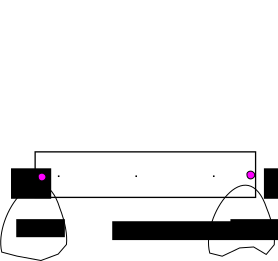
\includegraphics[scale=0.45]{./rep-landmarks.eps}
  %\vspace{-1ex}
  \caption{Using proxies for landmarks}
  \label{fig-angent-landmarks}
\end{minipage}
\begin{minipage}[b]{.24\textwidth}
  \centering
  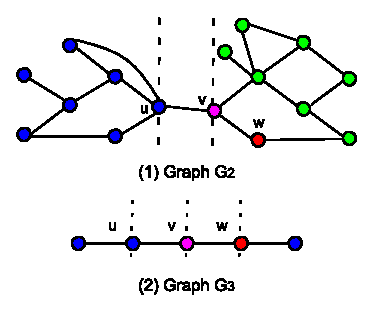
\includegraphics[scale=0.65]{./extended-proxies.eps}
  %\vspace{-1ex}
  \caption{Example proxies and \dras}
  \label{fig-proxies}
\end{minipage}%
\vspace{-4ex}
\end{figure}
}

\subsection{Routing Proxies and Deterministic Routing Areas}
\label{subsec-proxy-def}

We first present routing proxies and their deterministic routing areas.

\stitle{Proxies}. Given a node $u$ in graph $G(V, E)$, we say that $u$ is a {\em routing proxy} (or simply {\em proxy}) of a set of nodes, denoted by $A_{u}$, if and only if:
\sstab(1) node $u\in A_{u}$ is reachable to any node of $A_u$ in $G$,
\sstab(2) all neighbors of any node $v\in A_u\setminus \{u\}$ are in $A_u$,  and
\sstab(3) the size $|A_u|$ of $A_u$ is equal to or less than $c\cdot\lfloor\sqrt{|V|}\rfloor$, where $c$ is a small constant number, such as $2$ or $3$.


Here condition (1) guarantees the connectivity of subgraph $G[A_u]$,  condition (2) implies that not all neighbors of proxy $u$ are necessarily in $A_u$;
and condition (3), referred to as {\em size restriction}, limits the size of $A_u$ of proxy $u$.



Note that a node $u$ may be a proxy of multiple sets of nodes $A^1_u, \ldots, A^k_u$ such that $A^i_u\cap A^j_u$ = $\{u\}$ for any $i\ne j\in[1, k]$.
And we denote as $A^{+}_u$ the union of all the sets of nodes whose proxy is $u$ , \ie  $A^{+}_u$ = $A^1_u$ $\cup\ldots\cup$ $A^k_u$.

\stitle{Deterministic routing areas} . We refer to the {\em subgraph} $G[A^+_u]$ with nodes $A^+_u$ as a \dra of proxy $u$.

Intuitively, \dra $G[A^+_u]$ is a {\em maximal} connected subgraph connecting to the rest of graph $G$ through proxy $u$ only.

\stitle{Maximal proxies}.  We say that a proxy $u$ is {\em maximal} if there exist no other proxies $u'$ such that $A^+_{u} \subset A^+_{u'}$.

\stitle{Trivial proxies}. We say that a maximal proxy $u$ is {\em trivial} if $A^+_u$ contains itself only, \ie $A^+_{u}$ = $\{u\}$.


\stitle{Equivalent proxies}. We say that two proxies $u$ and $u'$ are {\em equivalent}, denoted by $u\equiv u'$, if $A^+_{u} = A^+_{u'}$.




We next illustrate these notions with an example below.

\begin{figure}
\centering
 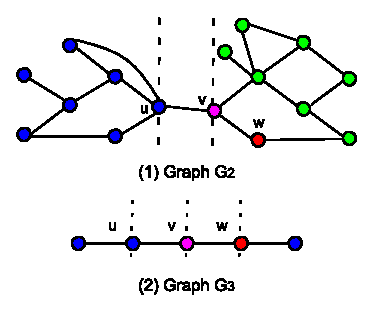
\includegraphics[scale=0.95]{./extended-proxies.eps}
 \vspace{-2ex}
 \caption{Example proxies and \dras}
  \label{fig-proxies}
\vspace{-2ex}
\end{figure}


\vspace{-0.5ex}
\begin{example}
\label{exm-proxies} First consider graph $G_2(V_2, E_2)$ in Fig.~\ref{fig-proxies}, and let $c\cdot\lfloor\sqrt{|V_2|}\rfloor$ =
$2\cdot\lfloor\sqrt{|16}\rfloor$ = $8$, where $c = 2$ and $|V_2| = 16$.
\sstab(1) Node $u$ is a proxy, and its \dra is the subgraph in the left hand side of the vertical line across $u$;
\sstab(2) Node $v$ is a proxy, and its \dra is the subgraph in the left hand side of the vertical line across $v$;
\sstab(3) Node $w$ is not a proxy since it can not find a \dra with size less or equal than $8$;
\sstab(4)  Node $v$ is a maximal proxy, while node $u$ is not a maximal proxy since $A^+_u\subset A^+_v$.


We then consider graph $G_3(V_3, E_3)$ in Fig.~\ref{fig-proxies}, and let $c\cdot\lfloor\sqrt{|V_3|}\rfloor$ =
$2\cdot\lfloor\sqrt{5|}\rfloor$ = $4$, where $c = 2$ and $|V_3| = 5$.
\sstab(1) Nodes $u, v$ and $w$ are three maximal proxies, whose \dras are all the entire graph $G_3$, and, hence,
\sstab(2) $u, v$ and $w$ are three equivalent proxies.
 \end{example}

\vspace{-1ex}
\stitle{Remark}. As illustrated by the above examples,  a \dra of graph $G(V, E)$ may have a size larger than $c\cdot\lfloor\sqrt{|V|}\rfloor$,
and multiple equivalent proxies.


We next show that proxies and \dras are {\em well defined} notions.


\begin{prop}
\label{prop-proxy-unique-dra} Any proxy in a graph has a unique \dra.
\end{prop}

\begin{proof}
We show this by contradiction. Assume first that there exists a proxy $u$ such that it has two distinct \dras: $G[A^+_{u,1}]$ and $G[A^+_{u,2}]$.
Then by the definition of \dra, it is trivial to verify the following:
%
\sstab(1) $A^+_{u,1}\not\subset A^+_{u,2}$,
\sstab(2) $A^+_{u,2}\not\subset A^+_{u,1}$, and
\sstab(3) $A^+_{u,1}\cap A^+_{u,2}$ has at least 2 nodes, and one must be $u$.

By the definition of proxy, $u$ is a proxy of all the set of nodes in $A^+_{u,1}\cup A^+_{u,2}$, and the \dra of $u$ should be $G[A^+_{u,1}\cup A^+_{u,2}]$. That is, neither $A^+_{u,1}$ nor $A^+_{u,2}$ is maximal. Hence, both $G[A^+_{u,1}]$ and $G[A^+_{u,2}]$ are not \dras of node $u$.
This contradicts to our previous assumption.
\end{proof}

\begin{prop}
\label{thm-proxy-disjoint} Given any two distinct proxies $u$ and $u'$, \\
(1) if $u\in A^+_{u'}$, then $A^+_{u}\subseteq A^+_{u'}$, \\
(2) if $u'\in A^+_{u}$, then $A^+_{u'}\subseteq A^+_{u}$,  and \\
(3) $A^+_{u}\cap A^+_{u'}$ = $\emptyset$, otherwise.
\end{prop}

\begin{proof}
Consider two distinct proxies $u$ and $u'$ in graph $G$.


(1) We first show that if $u\in A^+_{u'}$, then $A^+_{u}\subseteq A^+_{u'}$.

We show this by contradiction. Assume first that $A^+_{u}\not\subseteq A^+_{u'}$ and $u\in A^+_{u'}$.
Then there must exist a node $w\in A^+_{u}$, but $w\not\in A^+_{u'}$.
%
Since $w\in A^+_{u}$, by the definition of proxies, $w$ is reachable to $u$.
Moreover, since $u\in A^+_{u'}$, by the definition of proxies, all nodes reachable to $u$ belong to  $A^+_{u'}$
Hence, $w\in A^+_{u'}$, which contradicts our previous assumption.

(2) Similarly to (1), we can show that if $u'\in A^+_{u}$, then $A^+_{u'}\subseteq A^+_{u}$.

(3) For the case when $u\not\in A^+_{u'}$ and $u'\not\in A^+_{u}$, it is easy based on the analyses of (1) and (2).
\end{proof}

By Proposition~\ref{thm-proxy-disjoint}, it is easy to have the following, which says when maximal proxies are concerned, there exists a unique set of non-overlapping \dras.

\begin{cor}
\label{cor-proxy-disjoint} Given any two maximal proxies $u$ and $u'$, then either $A^+_{u} = A^+_{u'}$ or $A^+_{u}\cap A^+_{u'}$ = $\emptyset$ holds.
\end{cor}

\vspace{-1ex}
\stitle{Remark}. Trivial proxies only represent themselves, and, hence, we are only interested in non-trivial maximal proxies (or simply called proxies) in the sequel.


\subsection{Properties of Proxies and DRAs}
\label{subsec-proxy-properties}

We next give an analysis of proxies and \dras, and show that they hold good properties for shortest path and distance queries.
%
We first justify the necessity of the size restriction for proxies.  Otherwise, \dras are simply \ccs, and are mostly useless.


\begin{prop}
\label{prop-proxy-cc} Without the size restriction, any node $u$ in a graph $G$ is a maximal proxy,
and its \dra $G[A^+_u]$ is exactly the connected component (\cc) to which $u$ belongs.
\end{prop}

\begin{proof} Without loss of generality, we only consider those \ccs with at least two nodes.
Given any node $u$ in a graph $G$, by conditions (2) and (3) in the definition of proxy, there exists at least one neighbor $v$ of $u$ in $A^+_u$, and $A^+_u$ is not maximal, otherwise. By condition (2), all nodes reachable to $v$ are in $A^+_u$. It is known that all nodes in a \cc is reachable to any node in the \cc.
Hence, all nodes in a \cc belong to $A^+_u$. By these, we have the conclusion.
\end{proof}

The size restriction also guarantees that the shortest distance computation within a \dra can be evaluated efficiently,
as shown below.


\begin{prop}
\label{pro-proxy-path} Given any two nodes $v, v'$ in the \dra $G[A^+_u]$ of proxy $u$ in graph $G$, \\
(1) the shortest path in $G[A^+_u]$ is exactly the one in the entire graph $G$, and\\
(2) it can be computed in linear time in the size of $G$.
\end{prop}

\begin{proof} Consider a proxy $u$ in a graph, and two nodes $v$ and $v'$ in the \dra $G[A^+_u]$.
%
Let $G_s$ be the subgraph of removing $u$ from $G[A^+_u]$, and let $\cc_{1}$, $\ldots$, $\cc_{h}$ be the \ccs of $G_s$.
Observe that (a)  $G[A^+_{u}]$ is simply the union of all \ccs $\cc_{1}$, $\ldots$, $\cc_{h}$ and node $u$, and (b)
all \ccs have a size equal to or less than $c\cdot\lfloor\sqrt{|V|}\rfloor$ - $1$.  There are two cases to consider.

(1) Both nodes $v$ and $v'$ are in a single \cc $\cc_{j}$ ($1\le j\le h$).
Since \cc $\cc_{j}$ has no more than $c\cdot\lfloor\sqrt{|V|}\rfloor - 1$ nodes, it takes a standard Dijkstra algorithm at most $O(|V|)$ time to compute the shortest path between $v$ and $v'$.

(2) Nodes $v$ and $v'$ are in two distinct \ccs $\cc_{i}$ and $\cc_{j}$ ($1\le i\ne j\le h$).
As $u$ is the only node that $\cc_{i}$ and $\cc_{j}$ have in common, $\path(v,v')$ between $v$ and $v'$ is exactly $\path(v,u)$ + $\path(u,v')$, which can be computed in $O(|V|)$  time.

Putting these together, we have the conclusion.
\end{proof}

By Proposition~\ref{pro-proxy-path}, it is easy to derive the following.

\begin{cor}
\label{cor-proxy-distance} Given any two nodes $v, v'$ in the \dra $G[A^+_u]$ of proxy $u$ in graph $G$, \\
(1) the shortest distance $\dist(v, v')$ in $G[A^+_u]$ is exactly the one in the entire graph $G$, and\\
(2) it can be computed in linear time in the size of $G$.
\end{cor}


\begin{prop}
\label{pro-proxy-path-global} Given two nodes $v$ and $u$ with two distinct proxies $x$ and $y$, respectively, in graph $G$, the shortest path from $v$ to $u$ is $\path(v, x)$ $+$ $\path(x, y)$  $+$ $\path(y, u)$.
\end{prop}

\begin{proof}
We consider non-trivial maximal proxies. By its definition, (1) $v\neq x$ and $u\neq y$, (2) $v$ and $u$ are not neighboring nodes, (3)
for any node $w$ not in the \dra $G[A^+_{x}]$ of proxy $x$,  if $w$ is reachable to $v$, then $x$ must be a node in any shortest path from $w$ to $v$,
and, similarly, (4)  for any node $z$ not in the \dra $G[A^+_{y}]$ of proxy $y$,  if $z$ is reachable to $u$, then $y$ must be a node in any shortest path from $z$ to $y$.

This shows that the shortest path from $v$ to $u$ is exactly $\path(v, x)$ $+$ $\path(x, y)$  $+$ $\path(y, u)$.
\end{proof}


By Proposition~\ref{pro-proxy-path-global}, it is easy to derive the following result.

\begin{cor}
\label{cor-proxy-distance-global} Given two nodes $v$ and $u$ with two distinct proxies $x$ and $y$, respectively, in graph $G$, the shortest distance $\dist(v, u)$ = $\dist(v, x)$ $+$ $\dist(x, y)$  $+$ $\dist(y, u)$.
\end{cor}


Propositions~\ref{pro-proxy-path},~\ref{pro-proxy-path-global} and Corollaries~\ref{cor-proxy-distance},~\ref{cor-proxy-distance-global} guarantee that the shortest paths and distances between the nodes in the \dras of two distinct proxies can be answered in a correct and efficient way.


\begin{prop}
\label{prop-proxy-cut} Any proxy in a \cc $H(V_s, E_s)$ of graph $G(V$, $E)$ with $|V_s|>c\cdot\lfloor\sqrt{|V|}\rfloor$ must be a cut-node of graph $G$.
\end{prop}

\begin{proof} We show this by contradiction. We first assume that a proxy $u$ in a \cc $H(V_s, E_s)$ of graph $G(V$, $E)$ is not a cut-node.  Then we show that $u$ is not a proxy, a contradiction to our assumption.

Let $G\setminus\{u\}$ be the subgraph of $G$ by removing node $u$ from $G$.  Note that $G\setminus\{u\}$ remains connected since $u$ is not a cut node of graph $G$. By the definition of (non-trivial maximal) proxies, at least one neighbor $v$ of $u$ must belong to $A_{u}$.  As all nodes in $H\setminus\{u\}$ are reachable to $v$, it is easy to know that $A_{u}$ contains all the nodes $V_s$.  Since $|V_s| > c\cdot\lfloor\sqrt{|V|}\rfloor$, which violates the size condition of proxies. Hence, $u$ is not a proxy of $G$, which contradicts to our assumption.
\end{proof}


This motivates us to identify (non-trivial maximal) proxies by utilizing the cut-nodes and \bccs, which will be seen immediately.


\begin{prop}
\label{prop-large-bcc} Any node in a bi-connected component (\bc)  with size larger than $c\cdot\lfloor\sqrt{|V|}\rfloor$ of graph $G(V$, $E)$ is a trivial proxy.
\end{prop}

\begin{proof} We show this by contradiction.

Assume first that there exists a non-trivial proxy $u$ in a bi-connected component with size larger than $c \cdot\lfloor\sqrt{|V|}\rfloor$ of graph $G(V, E)$.
Then we show that $u$ is not a proxy. Let $G_s$ be the subgraph of the bi-connected component with the removal of $u$. Since the removal of any node in a \bc doesn't increase the number of \ccs, $G_s$ remains a \cc. By the definition of proxies, $A_u$ contains all the  the set of nodes in $G_s$ together with node $u$. That is, $A_u$ has more than $c \cdot\lfloor\sqrt{|V|}\rfloor$ nodes, and $u$ is not a proxy. This contradicts to our previous assumption.
\end{proof}

As we are interested in non-trivial proxies only, those large \bccs could be simply ignored without any side effects.



\subsection{Query Answering with Routing Proxies}
\label{subsec-proxy-query}


\begin{figure}[tb!]
%\vspace{-1ex}
\begin{center}
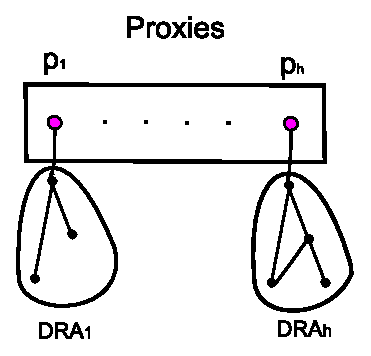
\includegraphics[scale=0.6]{./Proxy-framework.eps}
\end{center}
\vspace{-2ex}
\caption{Framework of using proxies}
\label{fig-angent-landmarks} \vspace{-2ex}
\end{figure}


 Based on the above analyses, we present a framework for speeding-up shortest  path and distance query answering, which consists of two modules: {\em preprocessing} and {\em query answering}. The framework for answering queries using proxies and \dras is illustrated in Fig.~\ref{fig-angent-landmarks}, in which each $p_i$ ($i\in[1, h]$) denotes a proxy, and is associated with its \dra. We next introduce the details of the framework.

\etitle{1. Preprocessing}. Given graph $G(V, E)$, the preprocessing module executes the following.

\noindent(1) It first computes the \dras and their maximal proxies,  using algorithm $\compDRAs$ (to be seen shortly in Section~\ref{sec-proxy-algorithms}).

\noindent(2) It then pre-computes and stores all the shortest paths and distances between any node in a \dra and its proxy.


\etitle{2. Query answering}. Given two nodes $s$ and $t$ in graph $G(V, E)$  and the pre-computed information, the query answering module executes the following.


\noindent(1) When nodes $s$ and $t$ belong to the same \dra $G[A^+_u]$ with proxy $u$ such that $A^+_u$ = $A^1_u\cup\ldots A^h_u$.

If $s$ and $t$ further fall into the same $A^i_u$ ($i\in[1,h]$), then it invokes the Dijkstra's algorithm on the subgraph $G[A^i_u]$ to compute the shortest path and distance between $s$ and $t$. Otherwise, it simply returns $\path(s, u)$ + $\path(u, t)$ or $\dist(s, u)$ + $\dist(u, t)$, in constant time.

\noindent(2)  When $s$ and $t$ belong to two \dras $G[A^+_{u_s}]$ and $G[A^+_{u_t}]$ with proxies $u_s$ and $u_t$, respectively.
%
Observe that $\path(s, t)$ = $\path(s, u_s)$ + $\path(u_s, u_t)$ + $\path(u_t, t)$ and $\dist(s, t)$ = $\dist(s, u_s)$ + $\dist(u_s, u_t)$ + $\dist(u_t, t)$, in which $\path(s, u_s)$, $\path(u_t, t)$, $\dist(s, u_s)$ and $\dist(u_t, t)$ are already known. Hence, it simply invokes an algorithm (\eg bidirectional Dijkstra~\cite{LubyR89}, \arcflag \cite{MohringSSWW05}, \ch~\cite{GeisbergerSSD08}, \tnr~\cite{bast2014route}) for computing $\path(u_s, u_t)$.
Similarly, the shortest distance $\dist(s, t)$ can be computed.

 Let $G'$ be the reduced subgraph of $G$ by removing all the nodes in \dras, but keeping their proxies, from graph $G$. It is easy to see that the main computation is reduced from $G$ to $G'$.   As shown in our experimental study (Section~\ref{sec-expt}), on average about 1/3 nodes of a graph are captured by non-trivial proxies and their \dras. That is, graph $G'$ is about 2/3 size of graph $G$, and hence our technique could reduce graph sizes and speed up shortest path and distance computations.
